%%%% 五号字对应10.5pt
\documentclass[10.5pt,twocolumn]{aaas}

%% 画圆圈数字
\newcommand*\circled[1]{\tikz[baseline=(char.base)]{
            \node[shape=circle,draw,inner sep=1pt] (char) {#1};}}

\newcommand\mycolorRed[1]{{\color{red}#1}}
\newcommand\mycolorYellow[1]{{\color{yellow}#1}}
\newcommand\mycolorBlue[1]{{\color{blue}#1}}

\DeclareMathSizes{10.5}{10}{6.8}{4.2}

%%% 设置公式前后距离
\setlength{\abovedisplayskip}{2.5mm}
\setlength{\belowdisplayskip}{2.5mm}

\clubpenalty=10000          % 禁止孤行
\widowpenalty=10000         % 禁止寡行

\usepackage{amsmath}
\usepackage{mathtools}
\usepackage{tabularx}
\usepackage{longtable}
\usepackage{makecell}
\renewcommand\cellgape{\Gape[-3pt][-3pt]}
\newcolumntype{Y}{>{\centering\arraybackslash}X}
\newcolumntype{L}{>{\raggedright\arraybackslash}X}

\usepackage{dashrule}
\usepackage{newtxmath}
\usepackage{placeins}

\usepackage{array}
\renewcommand\tabularxcolumn[1]{m{#1}}

\usepackage{tcolorbox}
\tcbuselibrary{breakable}

\InputIfFileExists{./private_identity.tex}{}{}
\providecommand{\PrivateAuthorNameCn}{佚名}
\providecommand{\PrivateAuthorNameEnAbbr}{YI M}
\providecommand{\PrivateAuthorNameEnFull}{YI Ming}
\providecommand{\PrivateAffiliationCn}{1.~~家里蹲大学~~摸鱼学院，北京~~100000}
\providecommand{\PrivateAffiliationEn}{1. School of Slacking, Stay-at-Home University, Beijing 100000, China}

\begin{document}

%%%%%%%%%%%%%%%%%%%%%%%%%%%%%%%%%%%%%%%%%%%%%%%%%%%%%%%%%%%%%%%%
% 标题、作者信息
%%%%%%%%%%%%%%%%%%%%%%%%%%%%%%%%%%%%%%%%%%%%%%%%%%%%%%%%%%%%%%%%
\title{
\vspace{2.39cm}{\CJKfontspec[Path = ./fonts/]{华文中宋.ttf}\xiaoerhao
基于{\TimesNMFont\textbf{Lambert}}转移与{\TimesNMFont\textbf{CW}}方程的共面抵近导引仿真
}\vspace{0.4cm}
}

\author{
{\kai\sihao \PrivateAuthorNameCn \makebox{$^{\text{1}}$}}\\[0.3cm]
{\fang\xiaowuhao \PrivateAffiliationCn}
}

\date{}

%%%%%%%%%%%%%%%%%%%%%%%%%%%%%%%%%%%%%%%%%%%%%%%%%%%%%%%%%%%%%%%%
% 中文摘要
%%%%%%%%%%%%%%%%%%%%%%%%%%%%%%%%%%%%%%%%%%%%%%%%%%%%%%%%%%%%%%%%
\CKeyword{空间抵近；Lambert转移；CW方程；多脉冲导引；绕飞轨道；LVLH坐标系}
\CLCNo{V448.234}
\Dcode{J}
\PaperNo{}

\twocolumn[
  \begin{@twocolumnfalse}
    \maketitle
    \positiontextbox{2.25cm}{4.3cm}{
    \liuhao
    \parbox{\textwidth}{%
    \hangindent=5em\hangafter=1
    {\CJKfontspec[FakeSlant = 0.2, FakeBold=2]{FangSong}  {\bfseries 引用格式：}}{ \CJKfontspec[FakeSlant = 0.2]{FangSong} \PrivateAuthorNameCn. 基于\textsl{Lambert}转移与\textsl{CW}方程的共面抵近导引仿真\textsl{[J]}. 航空学报, \textsl{2026, xx(x): XXXXXX. \PrivateAuthorNameEnAbbr.  Simulation of coplanar proximity guidance based on Lambert transfer and Clohessy-Wiltshire equations[J]. Acta Aeronautica et Astronautica Sinica, 2026, xx(x): XXXXXX(in Chinese). doi:}}%
    }}
    \begin{CAbstractAAAS}
      本文针对空间目标共面抵近任务，建立了由远程Lambert转移与近程CW（Clohessy-Wiltshire）多脉冲导引组成的分段设计方法。远程段在惯性系下基于二体动力学与Lambert理论，以出发时刻和飞行时间为搜索变量，并以转移弧段最低高度为安全约束，将跟踪飞行器由初始椭圆轨道导引至目标后方\SI{5}{km}捕获点。近程段在目标LVLH坐标系下，利用CW状态转移矩阵、直线指数趋近律和预设平面绕飞轨道切入条件，完成从捕获点到绕飞轨道的多脉冲转移设计。结果表明：远程段最优窗口对应出发时刻\SI{3960}{s}、飞行时间\SI{3300}{s}，总速度增量为\SI{262.9124}{m/s}，数值递推终点位置误差为\SI{0.001424}{m}；近程段在$N=2,3,4,5$的比较中，最优切入相位均位于第三象限，且随转移段数增加逐渐减小。虽然总速度增量由\SI{4.3442}{m/s}增至\SI{6.0034}{m/s}，但轨迹对参考直线的贴合程度持续改善，且增幅逐渐减小，因此本文选取$N=5$方案作为速度代价与轨迹形态折中下的推荐近程导引方案。本文结果验证了该分段导引策略在共面抵近场景下的有效性。
    \end{CAbstractAAAS}
  \end{@twocolumnfalse}
]

\wuhao

%%%%%%%%%%%%%%%%%%%%%%%%%%%%%%%%%%%%%%%%%%%%%%%%%%%%%%%%%%%%%%%%
% 正文
%%%%%%%%%%%%%%%%%%%%%%%%%%%%%%%%%%%%%%%%%%%%%%%%%%%%%%%%%%%%%%%%
% \section*{引言}

空间抵近任务是交会对接、近距离观测、在轨服务、目标抓捕和编队飞行等任务的基础环节。与单纯的轨道机动不同，抵近任务不仅要求飞行器进入目标附近区域，还要求在终端满足相对位置、相对速度和安全距离等约束。对于远距离段，飞行器之间的相对距离与地心轨道尺度相当，适合在惯性系中利用二体动力学和Lambert两点转移描述；对于近距离段，相对距离远小于目标轨道半径，可以在目标LVLH坐标系中利用线性相对运动模型，即CW（Clohessy-Wiltshire）方程，快速设计多脉冲导引律。

本文围绕共面抵近任务建立仿真方案。目标飞行器运行在离地\SI{1000}{km}高的圆轨道上，初始相位角为$80^\circ$。跟踪飞行器初始位于同一轨道平面内的椭圆轨道，近地点高度为\SI{400}{km}，远地点高度为\SI{600}{km}，初始真近点角为$45^\circ$。远程导引段的终端为目标后方\SI{5}{km}处捕获点。到达捕获点后，近距离导引段继续将跟踪飞行器切入预设平面绕飞轨道。目标平面绕飞轨道y轴偏置$y_\mathrm{const}=0$，径向幅值$k=1\si{km}$。

\section{理论模型}

\subsection{二体动力学与椭圆轨道时间推进}\label{subsec:orbit-time}

在忽略大气阻力、地球非球形摄动、第三体引力和连续推力作用的条件下，飞行器在地心惯性系中的运动由二体动力学描述：
\begin{equation}
  \ddot{\boldsymbol{r}}=-\mu\frac{\boldsymbol{r}}{r^3}
\end{equation}
其中$\boldsymbol{r}$为飞行器相对地心的位置矢量，$r$为位置矢量的模长，$\mu$为地球引力常数。

对于椭圆轨道，轨道几何方程为
\begin{equation}
  r=\frac{p}{1+e\cos\theta}=a\left(1-e\cos E\right)
\end{equation}
其中$e$为偏心率，$a$为半长轴，$\theta$为真近点角,$E$为偏近点角,$p=a(1-e^2)$为半通径。

偏近点角与真近点角的转换关系由下式给出：
\begin{equation}
  \theta=2\cdot\mathrm{atan2}\left(
  \sqrt{1+e}\sin\left(\frac{E}{2}\right),
  \sqrt{1-e}\cos\left(\frac{E}{2}\right)
  \right)
\end{equation}
\begin{equation}
  E=2\cdot\mathrm{atan2}\left(
  \sqrt{1-e}\sin\left(\frac{\theta}{2}\right),
  \sqrt{1+e}\cos\left(\frac{\theta}{2}\right)
  \right)
\end{equation}
其中$\mathrm{atan2}\left(\cdot\right)$为四象限反正切函数。

已知航天器的真近点角$\theta$，则其位置速度矢量由下式给出:
\begin{equation}
  \left\{
  \begin{aligned}
    \boldsymbol{r} & =
    r \begin{bmatrix}
        \cos \theta \\
        \sin \theta
      \end{bmatrix}
    \\
    \boldsymbol{v} & =
    \sqrt{\dfrac{\mu}{p}} \begin{bmatrix}
                            -\sin \theta \\
                            e+\cos \theta
                          \end{bmatrix}
  \end{aligned}
  \right.
\end{equation}

椭圆轨道的时间推进采用平近点角$M$：
\begin{equation}
  M(t)=M_0+n(t-t_0)
\end{equation}
其中平均角速度$n$为
\begin{equation}
  n=\sqrt{\frac{\mu}{a^3}}
\end{equation}
平近点角与偏近点角之间的关系由开普勒方程给出：
\begin{equation}
  E-e\sin E = M
\end{equation}


\subsection{Lambert两点转移}\label{subsec:lambert}

航天器任意时刻的位置速度矢量可由Lagrange系数与初始时刻位置速度矢量表示：
\begin{equation}
  \left\{
  \begin{aligned}
    \boldsymbol{r}(t)=f(t)\boldsymbol{r}_0+g(t)\boldsymbol{v}_0 \\
    \boldsymbol{v}(t)=\dot{f}(t)\boldsymbol{r}_0+\dot g(t)\boldsymbol{v}_0
  \end{aligned}
  \right.
\end{equation}
其中$f\dot{g}-\dot{f}g=1$。因此已知起止时刻的位置，转移弧段两端速度可表示为：
\begin{equation}\left\{
  \begin{aligned}
    \boldsymbol{v}_1=\frac{\boldsymbol{r}_2-f\boldsymbol{r}_1}{g} \\
    \boldsymbol{v}_2=\frac{\dot g\boldsymbol{r}_2-\boldsymbol{r}_1}{g}
  \end{aligned}
  \right.
  \label{eq:lambert-velocity}
\end{equation}
此时问题转化为求解$\eqref{eq:lambert-velocity}$中的Lagrange系数。

通用变量法可将Lambert问题转化为关于单个变量的时间方程。两位置矢量在轨道平面内的转移角为$\Delta\theta$。对于共面零圈转移，若起终点极角对应的逆时针夹角为$\phi_{\mathrm{ccw}}$，则几何短弧与长弧可分别写为
\begin{equation}
  \Delta\theta_{\mathrm{short}}
  =
  \min\left(\phi_{\mathrm{ccw}},2\pi-\phi_{\mathrm{ccw}}\right)
\end{equation}
\begin{equation}
  \Delta\theta_{\mathrm{long}}
  =
  2\pi-\Delta\theta_{\mathrm{short}}
\end{equation}
对给定分支，定义Lambert几何参数
\begin{equation}
  A=\sin\Delta\theta
  \sqrt{\frac{r_1r_2}{1-\cos\Delta\theta}}
\end{equation}
当$\Delta\theta$过小或$A$接近零时，两点转移几何趋于退化，标准Lambert速度关系不再具有良好的数值条件。

通用变量法的核心是把飞行时间约束写成关于单个变量$z$的隐式方程。先定义Stumpff函数
\begin{equation}
  C(z)=
  \begin{cases}
    \dfrac{1-\cos\sqrt{z}}{z},    & z>0 \\[1.0ex]
    \dfrac{1}{2},                 & z=0 \\[1.0ex]
    \dfrac{\cosh\sqrt{-z}-1}{-z}, & z<0
  \end{cases}
\end{equation}
\begin{equation}
  S(z)=
  \begin{cases}
    \dfrac{\sqrt{z}-\sin\sqrt{z}}{\left(\sqrt{z}\right)^3},     & z>0 \\[1.0ex]
    \dfrac{1}{6},                                               & z=0 \\[1.0ex]
    \dfrac{\sinh\sqrt{-z}-\sqrt{-z}}{\left(\sqrt{-z}\right)^3}, & z<0
  \end{cases}
\end{equation}
由$z$和几何参数$A$构造辅助函数
\begin{equation}
  y(z)=r_1+r_2+
  A\frac{zS(z)-1}{\sqrt{C(z)}}
\end{equation}
只有当$C(z)>0$且$y(z)>0$时，该$z$才对应可用的转移几何。进一步令
\begin{equation}
  \chi(z)=\sqrt{\frac{y(z)}{C(z)}}
\end{equation}
则给定飞行时间$\Delta t$的通用变量Lambert方程可写成隐式残差形式：
\begin{equation}
  F(z)=\chi^3(z)S(z)+A\sqrt{y(z)}
  -\sqrt{\mu}\Delta t=0
\end{equation}
对给定的$r_1$、$r_2$、$\Delta\theta$、$\Delta t$和$\mu$，满足该方程的$z$确定了相应的转移弧段。

求得$z$和$y(z)$后，Lagrange系数可由下式计算：
\begin{equation}\left\{
  \begin{aligned}
    f=1-\frac{y}{r_1}       \\
    g=A\sqrt{\frac{y}{\mu}} \\
    \dot g=1-\frac{y}{r_2}
  \end{aligned}
  \right.
\end{equation}
代入式(\ref{eq:lambert-velocity})得到转移起点速度$\boldsymbol{v}_{1,\mathrm{tr}}$和终点速度$\boldsymbol{v}_{2,\mathrm{tr}}$，进而可以求得转移所需的速度脉冲。

\subsection{LVLH坐标变换与CW方程}

近距离段采用目标飞行器LVLH坐标系。若目标惯性系状态为$(\boldsymbol{r}_t,\boldsymbol{v}_t)$，角动量为$\boldsymbol{h}_t = \boldsymbol{r}_t \times \boldsymbol{v}_t$，则LVLH系三轴单位矢量在惯性系下表示为
\begin{equation}\left\{
  \begin{aligned}
    \boldsymbol{e}_x & =\frac{\boldsymbol{r}_t}{\|\boldsymbol{r}_t\|} \\
    \boldsymbol{e}_z & =\frac{\boldsymbol{h}_t}{\|\boldsymbol{h}_t\|} \\
    \boldsymbol{e}_y & =\boldsymbol{e}_z \times \boldsymbol{e}_x
  \end{aligned}
  \right.
\end{equation}

LVLH系与惯性系之间的转换关系由旋转矩阵给出：

\begin{equation}
  \prescript{I}{}{\boldsymbol{R}}_{L} = \left(\prescript{L}{}{\boldsymbol{R}}_{I}\right)^\mathrm{T} =
  \begin{bmatrix}
    \boldsymbol{e}_x & \boldsymbol{e}_y & \boldsymbol{e}_z
  \end{bmatrix}
\end{equation}
\begin{equation}
  \frac{\mathrm{d}}{\mathrm{d}t}\left(\prescript{L}{}{\boldsymbol{R}}_{I}\right) =
  \boldsymbol{S}\left(\prescript{L}{}{\boldsymbol{\omega}}_{L,I}\right)
  \prescript{L}{}{\boldsymbol{R}}_{I}
\end{equation}
其中$\prescript{L}{}{\boldsymbol{\omega}}_{L,I}=[0,0,-n]^\mathrm{T}$是表示在LVLH系下惯性系相对于LVLH系的角速度，下文省略其角标；$\boldsymbol{S}(\cdot)$是叉乘算子的矩阵表示，即三维矢量对应的反对称矩阵。
对于任意矢量$\boldsymbol{x}$，使用左上角标标记所表示的坐标系，有转换关系如下：
\begin{equation}
  \prescript{L}{}{\boldsymbol{x}} = \prescript{L}{}{\boldsymbol{R}}_{I} \prescript{I}{}{\boldsymbol{x}}
\end{equation}
\begin{equation}
  \prescript{L}{}{\dot{\boldsymbol{x}}}
  = \frac{\mathrm{d}}{\mathrm{d}t}\left(\prescript{L}{}{\boldsymbol{R}}_{I} \prescript{I}{}{\boldsymbol{x}}\right)
  = \boldsymbol{\omega} \times \prescript{L}{}{\boldsymbol{x}} + \prescript{L}{}{\boldsymbol{R}}_{I} \prescript{I}{}{\dot{\boldsymbol{x}}}
\end{equation}

记$\boldsymbol{r},\boldsymbol{r}_t$为地心到两个航天器的矢量，$\boldsymbol{\xi},\dot{\boldsymbol{\xi}}$为LVLH系下的相对位置和速度矢量，于是有：
\begin{equation}
  \boldsymbol{\xi} = \prescript{L}{}{\boldsymbol{r}} - \prescript{L}{}{\boldsymbol{r}_t}
\end{equation}

\begin{equation}
  \dot{\boldsymbol{\xi}} = \prescript{L}{}{\dot{\boldsymbol{r}}} - \prescript{L}{}{\dot{\boldsymbol{r}}_t}
  = \omega \times \boldsymbol{\xi} + \prescript{L}{}{R}_{I} \left(\prescript{I}{}{\dot{\boldsymbol{r}}} - \prescript{I}{}{\dot{\boldsymbol{r}}_t}\right)
\end{equation}

当相对距离远小于目标轨道半径时，可将非线性相对运动方程线性化。设$\boldsymbol{\xi}=[x,y,z]^\mathrm{T}$，其中$x$、$y$、$z$分别为径向、沿迹和法向相对位置，$\boldsymbol{a}=[a_x,a_y,a_z]^\mathrm{T}$为LVLH坐标系中的控制加速度，则对于目标轨道为圆轨道的情形，有CW方程如下：
\begin{equation}
  \left\{
  \begin{aligned}
    \ddot x-2n\dot y-3n^2x & =a_x \\
    \ddot y+2n\dot x       & =a_y \\
    \ddot z+n^2z           & =a_z
  \end{aligned}
  \right.
\end{equation}
对于脉冲导引，两次脉冲之间令$\boldsymbol{a}=\boldsymbol{0}$，状态传播可写为
\begin{equation}
  \begin{bmatrix}
    \boldsymbol{\xi}(t) \\
    \dot{\boldsymbol{\xi}}(t)
  \end{bmatrix}
  =
  \begin{bmatrix}
    \Phi_{rr} & \Phi_{rv} \\
    \Phi_{vr} & \Phi_{vv}
  \end{bmatrix}
  \begin{bmatrix}
    \boldsymbol{\xi}_0 \\
    \dot{\boldsymbol{\xi}}_0
  \end{bmatrix}
\end{equation}
设$\tau=nt$，$s=\sin\tau$，$c=\cos\tau$，三维状态转移矩阵分块为
\begin{equation}
  \Phi_{rr}=
  \begin{bmatrix}
    4-3c      & 0 & 0 \\
    6(s-\tau) & 1 & 0 \\
    0         & 0 & c
  \end{bmatrix}
\end{equation}
\begin{equation}
  \Phi_{rv}=
  \begin{bmatrix}
    s/n      & 2(1-c)/n     & 0   \\
    2(c-1)/n & (4s-3\tau)/n & 0   \\
    0        & 0            & s/n
  \end{bmatrix}
\end{equation}
\begin{equation}
  \Phi_{vr}=
  \begin{bmatrix}
    3ns     & 0 & 0   \\
    6n(c-1) & 0 & 0   \\
    0       & 0 & -ns
  \end{bmatrix}
\end{equation}
\begin{equation}
  \Phi_{vv}=
  \begin{bmatrix}
    c   & 2s   & 0 \\
    -2s & 4c-3 & 0 \\
    0   & 0    & c
  \end{bmatrix}
\end{equation}

状态转移矩阵由转移时间$t$唯一决定，若在此基础上已知转移起止点，则可以求解出发时所需速度增量为：
\begin{equation}
  \Delta v = \left\|\dot{\boldsymbol{\xi}}_0^+ - \dot{\boldsymbol{\xi}}_0^-\right\|
  = \left\|\Phi_{rv}^{-1}\left(\boldsymbol{\xi}_t - \Phi_{rr}\boldsymbol{\xi}_0 \right)-\dot{\boldsymbol{\xi}}_0^-\right\|
  \label{eq:segment-impulse}
\end{equation}

对于多脉冲转移，设节点序列为$\{\boldsymbol{\xi}_m\}_{m=0}^{N}$，总转移时间为$T$，各段时间间隔为$\Delta t_s=T/N$。此处$\Phi_{rr}$、$\Phi_{rv}$、$\Phi_{vr}$和$\Phi_{vv}$均取传播时间$\Delta t_s$。对第$m$段，令段首脉冲前后的相对速度分别为$\dot{\boldsymbol{\xi}}_m^-$与$\dot{\boldsymbol{\xi}}_m^+$，则由CW状态转移矩阵可得
\begin{equation}
  \dot{\boldsymbol{\xi}}_m^+
  = \Phi_{rv}^{-1}\left(\boldsymbol{\xi}_{m+1} - \Phi_{rr}\boldsymbol{\xi}_m\right)
  \quad m=0,1,\ldots,N-1
  \label{eq:multi-impulse-post-velocity}
\end{equation}
相应的段首脉冲为
\begin{equation}
  \Delta\boldsymbol{v}_m
  = \dot{\boldsymbol{\xi}}_m^+ - \dot{\boldsymbol{\xi}}_m^-
  \qquad m=0,1,\ldots,N-1
  \label{eq:multi-impulse-segment-dv}
\end{equation}
该段无控传播结束时的段末速度递推为
\begin{equation}
  \dot{\boldsymbol{\xi}}_{m+1}^-
  = \Phi_{vr}\boldsymbol{\xi}_m + \Phi_{vv}\dot{\boldsymbol{\xi}}_m^+
  \qquad m=0,1,\ldots,N-1
  \label{eq:multi-impulse-velocity-recursion}
\end{equation}
若目标绕飞轨道切入点要求的相对速度为$\dot{\boldsymbol{\xi}}_f$，则末端切入脉冲与多脉冲总速度增量分别为
\begin{equation}
  \Delta\boldsymbol{v}_{\mathrm{ins}}
  = \dot{\boldsymbol{\xi}}_f - \dot{\boldsymbol{\xi}}_N^-
  \label{eq:proximity-insertion-dv}
\end{equation}
\begin{equation}
  \Delta V_{\mathrm{prox}}
  = \sum_{m=0}^{N-1}\left\|\Delta\boldsymbol{v}_m\right\|
  + \left\|\Delta\boldsymbol{v}_{\mathrm{ins}}\right\|
  \label{eq:proximity-total-dv}
\end{equation}

\subsection{CW方程下的椭圆绕飞轨道}

在无控条件下，CW方程存在一类相对于目标飞行器周期闭合的自然绕飞轨道。首先将CW方程解析解改写为长期项与周期项的形式为
\begin{equation}
  \left\{
  \begin{aligned}
    x & =x_{\mathrm{const}}+k\sin (nt+\alpha)                                   \\
    y & =y_{\mathrm{const}}-\frac{3}{2}ntx_{\mathrm{const}} +2k\cos (nt+\alpha) \\
    z & =m\sin(nt+\beta)
  \end{aligned}\right.
\end{equation}
令$x_\mathrm{const}=0$，可消除其中长期项，得到平面周期解为
\begin{equation}
  \left\{
  \begin{aligned}
    x & =k\sin(nt+\alpha)                    \\
    y & =2k\cos(nt+\alpha) +y_\mathrm{const} \\
    z & =m\sin(nt+\beta)
  \end{aligned}
  \right.
  \label{eq:fly-around-orbit}
\end{equation}
式中，$k$为径向幅值，$y_\mathrm{const}$为沿迹方向中心偏置。该绕飞轨道的面内轨迹与面外轨迹独立，各由两个参数决定。
对于本文的共面算例，仅考虑平面绕飞轨道，因此取$m=0$。此时切入点状态由$k$、$y_\mathrm{const}$和切入相位$\theta_{\mathrm{in}}$确定。

\section{远程段导引策略与结果}

\subsection{Lambert窗口搜索策略}

远程段导引目标是将跟踪飞行器从初始椭圆轨道转移到目标后方捕获点，并在到达时满足零相对速度条件。该段采用出发与到达两次脉冲，通过对出发时刻$t_d$和飞行时间$\Delta t$进行窗口搜索，获得满足安全约束且速度增量较小的转移方案。远程段窗口搜索参数列于表\ref{tab:remote-search-params}。

对每一组$(t_d,\Delta t)$，先由\ref{subsec:orbit-time}节中的椭圆轨道时间函数计算跟踪飞行器出发状态$(\boldsymbol{r}_1,\boldsymbol{v}_{1,\mathrm{nom}})$与到达状态$(\boldsymbol{r}_2,\boldsymbol{v}_{f})$，随后使用\ref{subsec:lambert}节中的Lambert理论公式基于数值方法求解转移弧段两端速度$\boldsymbol{v}_{1,\mathrm{tr}}$和$\boldsymbol{v}_{2,\mathrm{tr}}$，最后使用总速度增量作为评价函数，定义为
\begin{equation}
  J = \Delta v_1 + \Delta v_2
  =
  \left\|\boldsymbol{v}_{1,\mathrm{tr}}-\boldsymbol{v}_{1,\mathrm{nom}}\right\|
  +
  \left\|\boldsymbol{v}_f-\boldsymbol{v}_{2,\mathrm{tr}}\right\|
\end{equation}

\begin{table}[t!]
  \centering
  \captionnamefont{\xiaowuhao\bf}
  \captiontitlefont{\xiaowuhao\bf}
  \bicaption[tab:remote-search-params]{表}{远程段窗口搜索参数}{Table}{Search parameters of the remote-guidance window}
  \liuhao
  \begin{tabularx}{0.98\columnwidth}{LLL}
    \hline
    参数           & 含义          & 取值                      \\
    \hline
    $t_d$        & 出发时刻        & $[0,1.5T_t]$            \\
    $\Delta t$   & Lambert飞行时间 & $[\SI{10}{min},1.2T_t]$ \\
    $\Delta t_g$ & 网格步长        & \SI{60}{s}              \\
    安全阈值         & 转移弧段最低半径下限  & $R_e+\SI{150}{km}$      \\
    \hline
  \end{tabularx}
\end{table}

\subsection{结果分析}

\begin{figure}[t!]
  \centering
  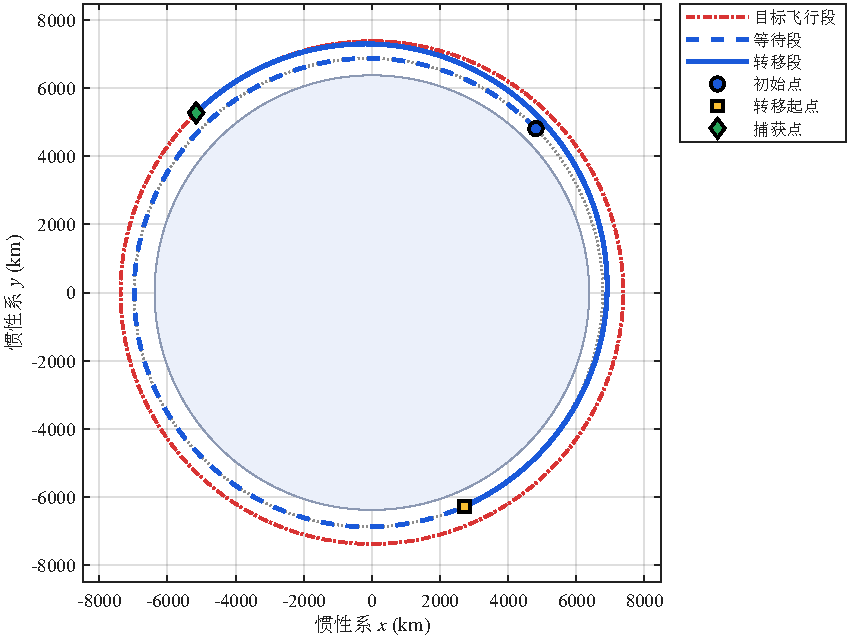
\includegraphics[width=3in]{./image/最优 Lambert 转移轨迹.pdf}
  \bicaption[fig:remote-trajectory]{图}{\centering 最优远程导引转移轨迹}{Fig.}{\centering Optimal transfer trajectory of the remote-guidance phase}
\end{figure}


在满足表\ref{tab:remote-search-params}所列安全阈值的候选网格中，搜索得到的最优Lambert窗口见表\ref{tab:remote-results}。图\ref{fig:remote-trajectory}展示了跟踪飞行器的等待与转移轨迹，该最优方案先沿初始椭圆轨道完成一段等待飞行，随后在轨道下半部实施转移脉冲，并沿位于目标圆轨道内侧的Lambert弧段飞向目标后方捕获点。由图中几何关系可以看出，转移段始终保持在目标轨道内侧推进，且捕获点位于目标运动轨迹后方。进一步在惯性系中对整个转移过程进行数值递推后，终点位置误差为\SI{0.001424}{m}，说明解析设计与数值仿真结果一致。

图\ref{fig:remote-contour}给出了$t_d-\Delta t$平面上的总速度增量等高线分布。可以看出，可行解并非大范围平坦区域，而是在某以局部最优解附近附近形成了较为集中的低值盆地。进一步将出发时刻整体后移并扩大搜索区间后，如图\ref{fig:remote-contour-2}所示出现了另一个形态相近的可行窗口，说明该类低值窗口会随目标与跟踪器相对相位的演化周期性重复出现；与此同时，由于跟踪器初始轨道为椭圆轨道，不同窗口对应的出发几何并不完全相同，因此等高线的外形和局部最优值仍存在一定差异。

同时，本文在不考虑目标航天器抵近目标的前提下，对跟踪航天器由初始轨道向目标航天器所在圆轨道的两脉冲转移策略进行了搜索，得到的最优方案总速度增量为\SI{262.7648}{m/s}，与表\ref{tab:remote-results}中的结果相近，说明考虑抵近任务目标并未引入过大的额外代价。

\begin{table}[t!]
  \centering
  \captionnamefont{\xiaowuhao\bf}
  \captiontitlefont{\xiaowuhao\bf}
  \bicaption[tab:remote-results]{表}{\centering 远程段Lambert窗口搜索结果记录}{Table}{\centering Result record of Lambert window search in the remote-guidance phase}
  \liuhao
  \begin{tabularx}{0.98\columnwidth}{LL}
    \hline
    指标               & 数值                 \\
    \hline
    最优出发时刻$t_d$      & \SI{3960.00}{s}    \\
    最优飞行时间$\Delta t$ & \SI{3300.00}{s}    \\
    出发脉冲$\Delta v_1$ & \SI{117.4185}{m/s} \\
    到达脉冲$\Delta v_2$ & \SI{145.4939}{m/s} \\
    总速度增量$\Delta V$  & \SI{262.9124}{m/s} \\
    数值递推终点位置误差       & \SI{0.001424}{m}   \\
    \hline
  \end{tabularx}
\end{table}


\begin{figure}[t!]
  \centering
  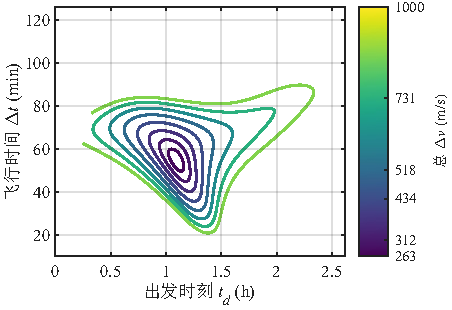
\includegraphics[]{./image/远程导引 Lambert 窗口等高线图.pdf}
  \bicaption[fig:remote-contour]{图}{\centering 远程导引Lambert窗口等高线图}{Fig.}{\centering Contour map of Lambert transfer windows in the remote-guidance phase}
\end{figure}

\begin{figure}[t!]
  \centering
  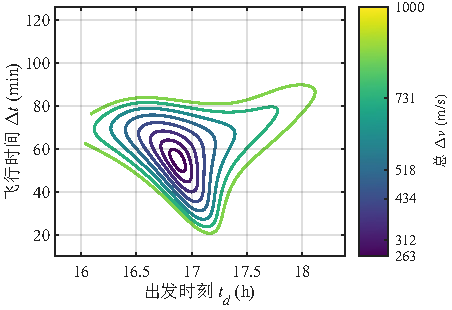
\includegraphics[]{./image/远程导引 Lambert 窗口等高线图2.pdf}
  \bicaption[fig:remote-contour-2]{图}{\centering 出发时间延后的另一个转移窗口等高线图}{Fig.}{\centering Contour map of another Lambert transfer window with delayed departure in the remote-guidance phase}
\end{figure}


\begin{figure}[t!]
  \centering
  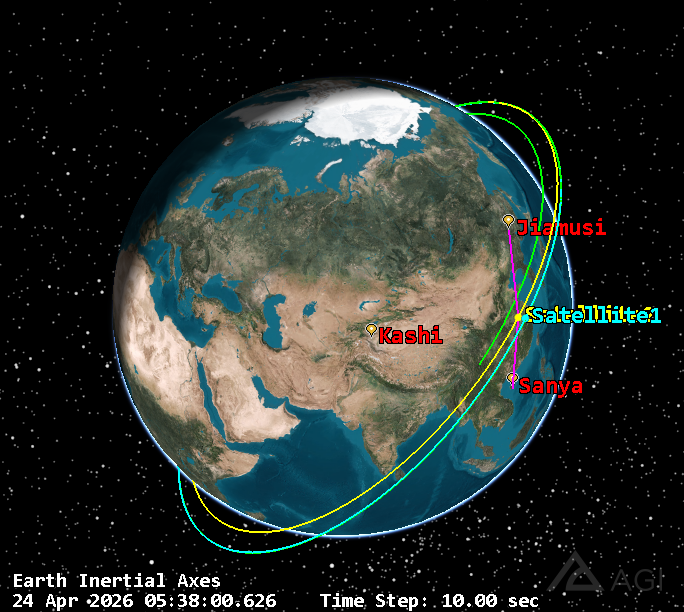
\includegraphics[width=3in]{./image/STK-R-2.png}
  \bicaption[fig:stk-scene]{图}{\centering STK仿真场景}{Fig.}{\centering STK simulation scenario}
\end{figure}


\subsection{STK可视化仿真}

本文将求解得出的最优Lambert转移方案输入到STK (Systems Tool Kit) 中进行可视化仿真，如图\ref{fig:stk-scene}所示，设置了三个地面站，分别为喀什、佳木斯、三亚，限制水平仰角大于8度。

图\ref{fig:stk-remote}展示了飞行器的三维轨迹，与前述解析结果一致。图\ref{fig:stk-elements}展示了等待与转移过程中跟踪飞行器的轨道根数变化，脉冲机动主要引起半长轴、近地点幅角和平近点角的分段变化，而轨道倾角和升交点赤经基本保持不变，这与本文共面远程转移的建模假设一致。图\ref{fig:stk-access}展示了地面站可见数量相对于时间的变化，地面站对转移过程的观测表现为若干离散可见窗口，这说明远程段运行过程中对测控时序仍需结合轨道位置统筹安排。

同时，本文还进行了接近分析与光照条件分析。图\ref{fig:stk-CAT-warning}展示了飞行器在转移截断与其他飞行物的接近告警情况，接近告警时刻在整个仿真时段内呈离散分布，最近接近距离处于数公里量级，需要考虑并优化设计。图\ref{fig:stk-eclipse}展示了跟踪飞行器的光照条件变化，其随轨道位置呈周期性变化，因此远程段任务若叠加光学观测或能源约束，还需要进一步联合考虑光照条件。


\begin{figure}[t!]
  \centering
  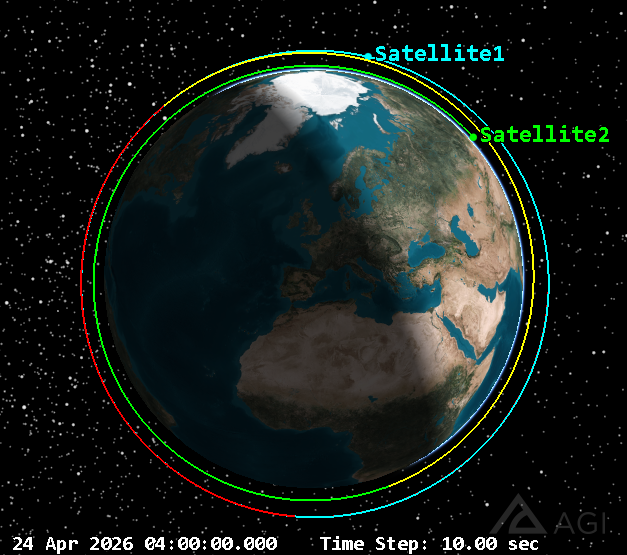
\includegraphics[width=3in]{./image/STK-R-1.png}
  \bicaption[fig:stk-remote]{图}{\centering STK远程导引可视化仿真轨迹}{Fig.}{\centering Visualization of the remote-guidance transfer trajectory in STK}
\end{figure}

\begin{figure}[t!]
  \centering
  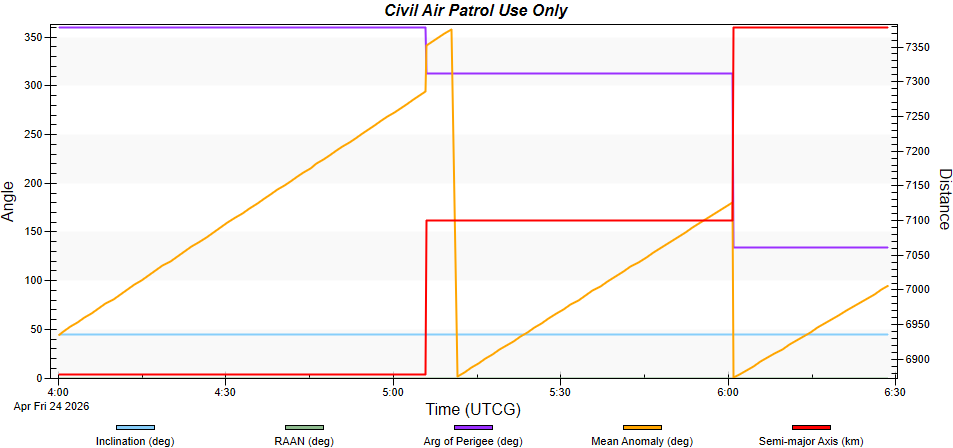
\includegraphics[width=3in]{./image/Satellite2_Classical_Orbit_Elements.png}
  \bicaption[fig:stk-elements]{图}{\centering 跟踪航天器轨道根数变化}{Fig.}{\centering Variation of the tracking spacecraft's classical orbital elements}
\end{figure}

\begin{figure}[t!]
  \centering
  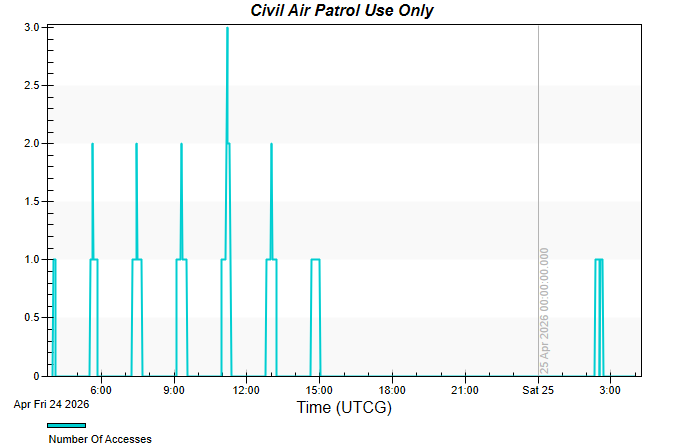
\includegraphics[width=3in]{./image/Chain1_Number_Of_Accesses.png}
  \bicaption[fig:stk-access]{图}{\centering 地面站可观测性}{Fig.}{\centering Ground station visibility of the transfer trajectory in STK}
\end{figure}

\begin{figure}[t!]
  \centering
  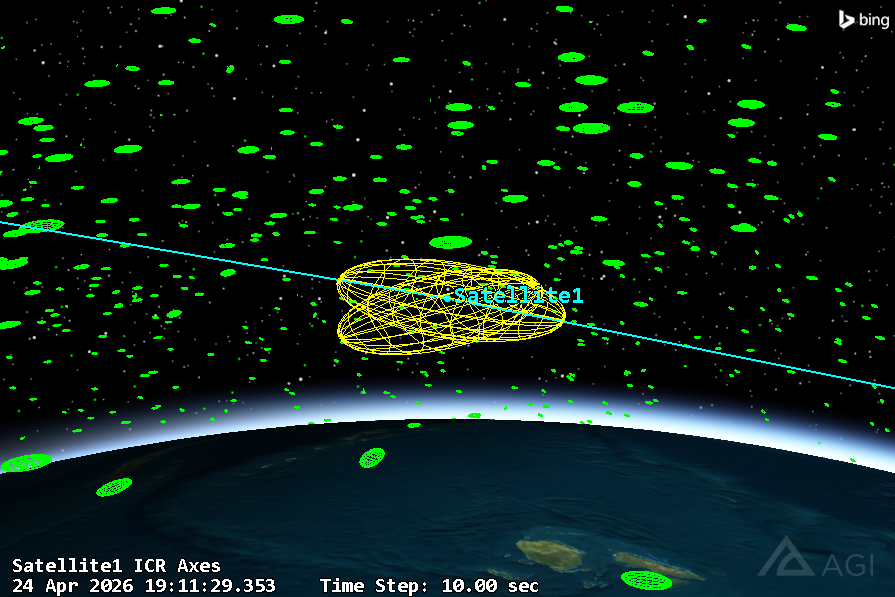
\includegraphics[width=3in]{./image/STK-R-3.png}
  \bicaption[fig:stk-CAT]{图}{\centering 航天器接近分析场景}{Fig.}{\centering Visualization of the close approach tool in STK}
\end{figure}

\begin{figure}[t!]
  \centering
  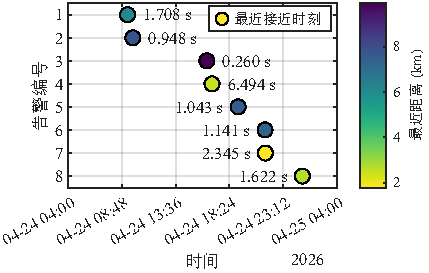
\includegraphics[width=3in]{./image/STK AdvCAT 接近告警时刻.pdf}
  \bicaption[fig:stk-CAT-warning]{图}{\centering 接近告警时刻}{Fig.}{\centering Close approach warning time of the spacecraft}
\end{figure}

\begin{figure}[t!]
  \centering
  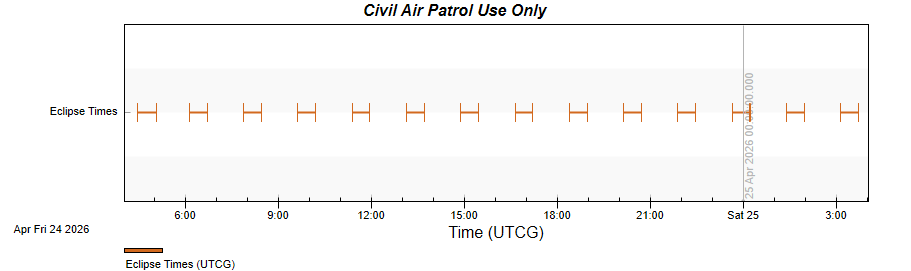
\includegraphics[width=3in]{./image/Satellite2_Eclipse_Times.png}
  \bicaption[fig:stk-eclipse]{图}{\centering 航天器光照条件变化}{Fig.}{\centering Variation of the tracking spacecraft's eclipse times}
\end{figure}

\section{近程段导引策略与结果}


\subsection{直线指数趋近律设计}

直线脉冲路径是一种经典的抵近模式，其在航天器与目标之间构造一条直线轨迹，并在其上选取多个脉冲节点进行速度修正。记抵近反方向的单位矢量为：

\begin{equation}
  \hat{\boldsymbol{\rho}} = \frac{\boldsymbol{\xi}_0-\boldsymbol{\xi}_T}{\left\|\boldsymbol{\xi}_0-\boldsymbol{\xi}_T\right\|}
\end{equation}
则每次脉冲位置与时间可以描述为：
\begin{equation}
  \left\{
  \begin{aligned}
    \boldsymbol{\xi}_m & = \boldsymbol{\xi}_T + \rho(t_m)\hat{\boldsymbol{\rho}} \\
    t_m                & = \frac{mT}{N},\quad m=1,2,\ldots,N-1
  \end{aligned}
  \right.
  \label{eq:approach-node}
\end{equation}


\begin{table*}[t!]
  \centering
  \captionnamefont{\xiaowuhao\bf}
  \captiontitlefont{\xiaowuhao\bf}
  \bicaption[tab:prox-results]{表}{不同转移段数下近距离导引最优方案结果记录}{Table}{Optimal proximity-guidance results under different transfer segment numbers}
  \liuhao
  \begin{tabularx}{0.96\textwidth}{
      >{\hsize=2.0\hsize\raggedright\arraybackslash}X
      >{\hsize=0.75\hsize\centering\arraybackslash}X
      >{\hsize=0.75\hsize\centering\arraybackslash}X
      >{\hsize=0.75\hsize\centering\arraybackslash}X
      >{\hsize=0.75\hsize\centering\arraybackslash}X
    }
    \hline
    指标（单位）                                     & $N=2$                                   & $N=3$  & $N=4$  & $N=5$  \\
    \hline
    起点趋近速率$\dot{\rho}_0$（\si{m/s}）             & -1.857                                  & -1.857 & -1.857 & -1.5   \\
    终点趋近速率$\dot{\rho}_T$（\si{m/s}）             & -1.371                                  & -1.371 & -1.243 & -1.371 \\
    总转移时间$T$（\si{min}）                         & 39.75                                   & 39.75  & 39.83  & 39.88  \\
    最优切入相位$\theta_{\mathrm{in}}$（\si{\degree}） & 231                                     & 231    & 225    & 216    \\
    脉冲序列（\si{m/s}）                             & 1.70 / 1.79 / 0.85
                                               & 1.81 / 1.76 / 1.06 / 0.64
                                               & 1.81 / 1.53 / 1.08 / 0.69 / 0.64
                                               & 1.52 / 1.17 / 0.99 / 0.81 / 0.64 / 0.87                            \\
    总速度增量$\Delta V_{\mathrm{prox}}$（\si{m/s}）  & 4.3442                                  & 5.2603 & 5.7474 & 6.0034 \\
    单次脉冲最大值（\si{m/s}）                          & 1.7942                                  & 1.8057 & 1.8091 & 1.5180 \\
    单次脉冲最小值（\si{m/s}）                          & 0.8503                                  & 0.6405 & 0.6443 & 0.6437 \\
    \hline
  \end{tabularx}
\end{table*}



通过设计相对位置的衰减函数$\rho(t)$，可以对抵近轨道进行设计。指数趋近律设定抵近函数满足
\begin{equation}
  \dot{\rho}=a\rho+\dot{\rho}_T
\end{equation}
给定初值条件$\dot{\rho}(0)=\dot{\rho}_0$，可解得
\begin{equation}
  a=\frac{\dot{\rho}_0-\dot{\rho}_T}{\rho_0}
\end{equation}
求解可得
\begin{equation}
  \label{eq:rho-func}
  \rho(t)=\rho_0 e^{at} + \frac{\dot{\rho}_T}{a}\left(e^{at}-1\right)
\end{equation}
由终端条件$\rho(T)=0$，可求得总转移时间为
\begin{equation}
  \label{eq:rho-T}
  T=\frac{\ln(\dot{\rho}_T/\dot{\rho}_0)}{a}
\end{equation}


对于本文的任务场景，设计参数共有四个：转移段数$N$、初始趋近速率$\dot{\rho}_0$、终端趋近速率$\dot{\rho}_T$和绕飞轨道切入点相位$\theta_{\mathrm{in}}$。

对于给定的趋近速率边界条件$\dot{\rho}_0$和$\dot{\rho}_T$，可以通过式\eqref{eq:rho-T}与\eqref{eq:rho-func}计算得到趋近函数$\rho(t)$和总转移时间$T$。进一步给定转移段数$N$和切入点相位$\theta_{\mathrm{in}}$，可以由式\eqref{eq:fly-around-orbit}计算得到切入点位置速度，并由式\eqref{eq:approach-node}生成每个转移段的节点位置。随后依据式\eqref{eq:multi-impulse-post-velocity}--\eqref{eq:multi-impulse-velocity-recursion}逐段反解脉冲与传播速度，并按式\eqref{eq:proximity-insertion-dv}与\eqref{eq:proximity-total-dv}计算末端切入脉冲和总速度增量。



\subsection{结果分析}

\begin{figure}[t!]
  \centering
  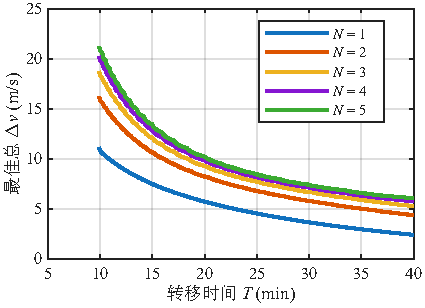
\includegraphics[]{./image/近距离导引转移时间-最佳总速度增量关系图.pdf}
  \bicaption[fig:prox-dv-time]{图}{\centering 近程导引转移时间与最佳总速度增量关系}{Fig.}{\centering Relationship between transfer time and the optimal total velocity increment in the proximity-guidance phase}
\end{figure}

\begin{figure*}[t!]
  \centering
  \subfigure[$N=2$]{
    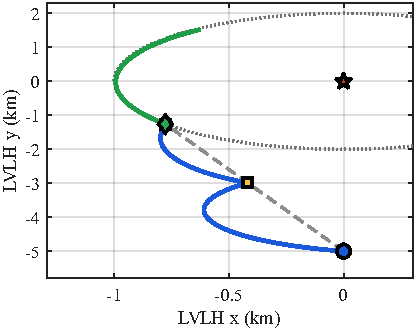
\includegraphics[width=0.235\textwidth]{./image/近距离导引相对系轨迹2.pdf}
  }%
  \hfill
  \subfigure[$N=3$]{
    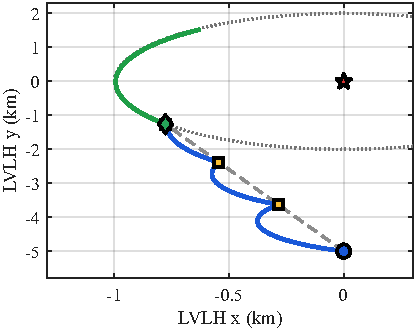
\includegraphics[width=0.235\textwidth]{./image/近距离导引相对系轨迹3.pdf}
  }%
  \hfill
  \subfigure[$N=4$]{
    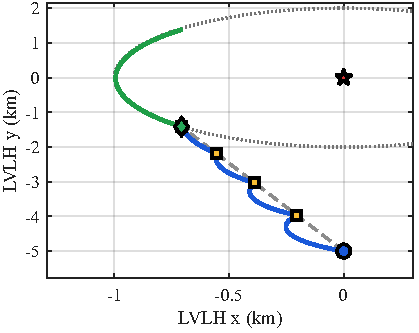
\includegraphics[width=0.235\textwidth]{./image/近距离导引相对系轨迹4.pdf}
  }%
  \hfill
  \subfigure[$N=5$]{
    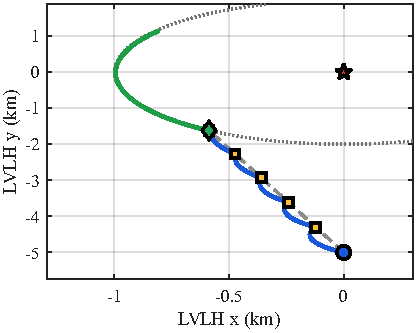
\includegraphics[width=0.235\textwidth]{./image/近距离导引相对系轨迹5.pdf}
  }
  \bicaption[fig:prox-trajectory]{图}{\centering 近程多脉冲转移与绕飞轨迹}{Fig.}{\centering Trajectories of proximity multi-impulse transfer and fly-around motion}
\end{figure*}


\begin{figure*}[t!]
  \centering
  \subfigure[$N=2$]{
    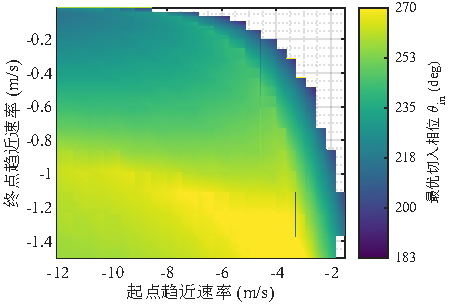
\includegraphics[width=0.235\textwidth]{./image/近距离导引起止调度导数归并最优切入相位颜色图2.pdf}
  }
  \hfill
  \subfigure[$N=3$]{
    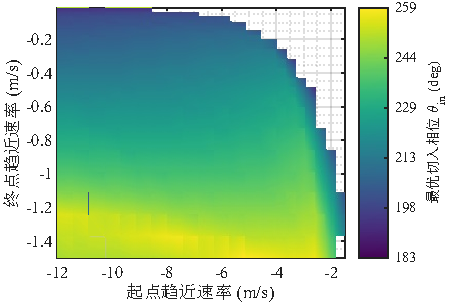
\includegraphics[width=0.235\textwidth]{./image/近距离导引起止调度导数归并最优切入相位颜色图3.pdf}
  }
  \hfill
  \subfigure[$N=4$]{
    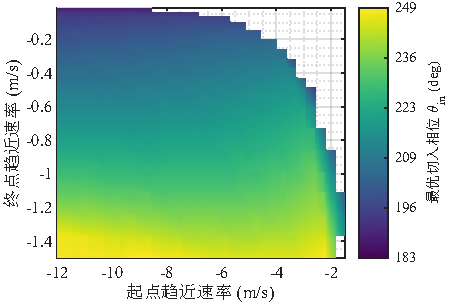
\includegraphics[width=0.235\textwidth]{./image/近距离导引起止调度导数归并最优切入相位颜色图4.pdf}
  }
  \hfill
  \subfigure[$N=5$]{
    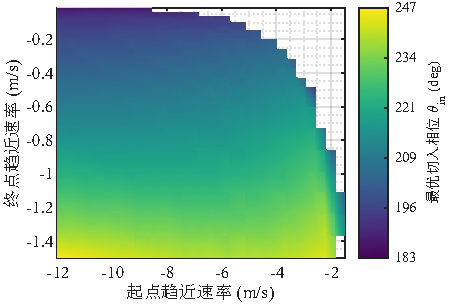
\includegraphics[width=0.235\textwidth]{./image/近距离导引起止调度导数归并最优切入相位颜色图5.pdf}
  }
  \bicaption[fig:prox-insert-theta]{图}{\centering 近程多脉冲转移最优切入相位分布}{Fig.}{\centering Distribution of the optimal insertion phase for the proximity multi-impulse transfer}
\end{figure*}

图\ref{fig:prox-dv-time}展示了不同转移时间所对应的最佳速度脉冲变化趋势，随着转移时间的增大，最优总速度增量单调下降，搜索过程中$\dot{\rho}_0$与$\dot{\rho}_T$往往落在使总转移时间接近上限的边界组合附近，主要需要搜索的变量为切入点相位$\theta_{\mathrm{in}}$。考虑到CW方程建立在线性化假设基础上，转移时间过长可能会导致线性化误差积累，因此本文将总转移时间限制在$\SI{40}{min}$以内，以保证设计结果的合理性。

本文分别对转移段数$N=2,3,4,5$的情况进行了搜索，得到的最优转移轨迹见图\ref{fig:prox-trajectory}，相关结果记录在表\ref{tab:prox-results}中。从图中可以看出，各方案均由目标后方\SI{5}{km}捕获点出发，并最终切入参考平面绕飞轨道；当转移段数较少时，转移弧段弯曲更明显，节点之间的修正幅度较大，而随着转移段数增加，节点逐渐增多，轨迹整体更贴近设计直线方向，表现为通过多次小幅速度修正逐步逼近切入点。与之对应，总速度增量由$N=2$时的\SI{4.3442}{m/s}逐步增加到$N=5$时的\SI{6.0034}{m/s}，但相邻方案的增量分别约为\SI{0.9161}{m/s}、\SI{0.4871}{m/s}和\SI{0.2560}{m/s}，呈现出明显的增幅趋缓特征。综合考虑速度代价与轨迹形态，$N=5$方案虽然脉冲略有上升，但其轨迹最贴合参考直线，因此本文将其作为近程段的推荐方案。

最优切入点相位的结果见图\ref{fig:prox-insert-theta}。由图可见，不同$N$下的最优切入相位均集中在第三象限，且在可行域内部呈连续分布，而不是离散跳变。随着起点与终点趋近速率的组合变化，最优相位在第三象限内平滑移动；当转移段数由$N=2$增大到$N=5$时，整幅分布整体向较小相位方向偏移，这与表\ref{tab:prox-results}中最优切入相位由$231^\circ$逐步减小到$216^\circ$的结果一致。

\subsection{STK可视化仿真}


\begin{figure}[t!]
  \centering
  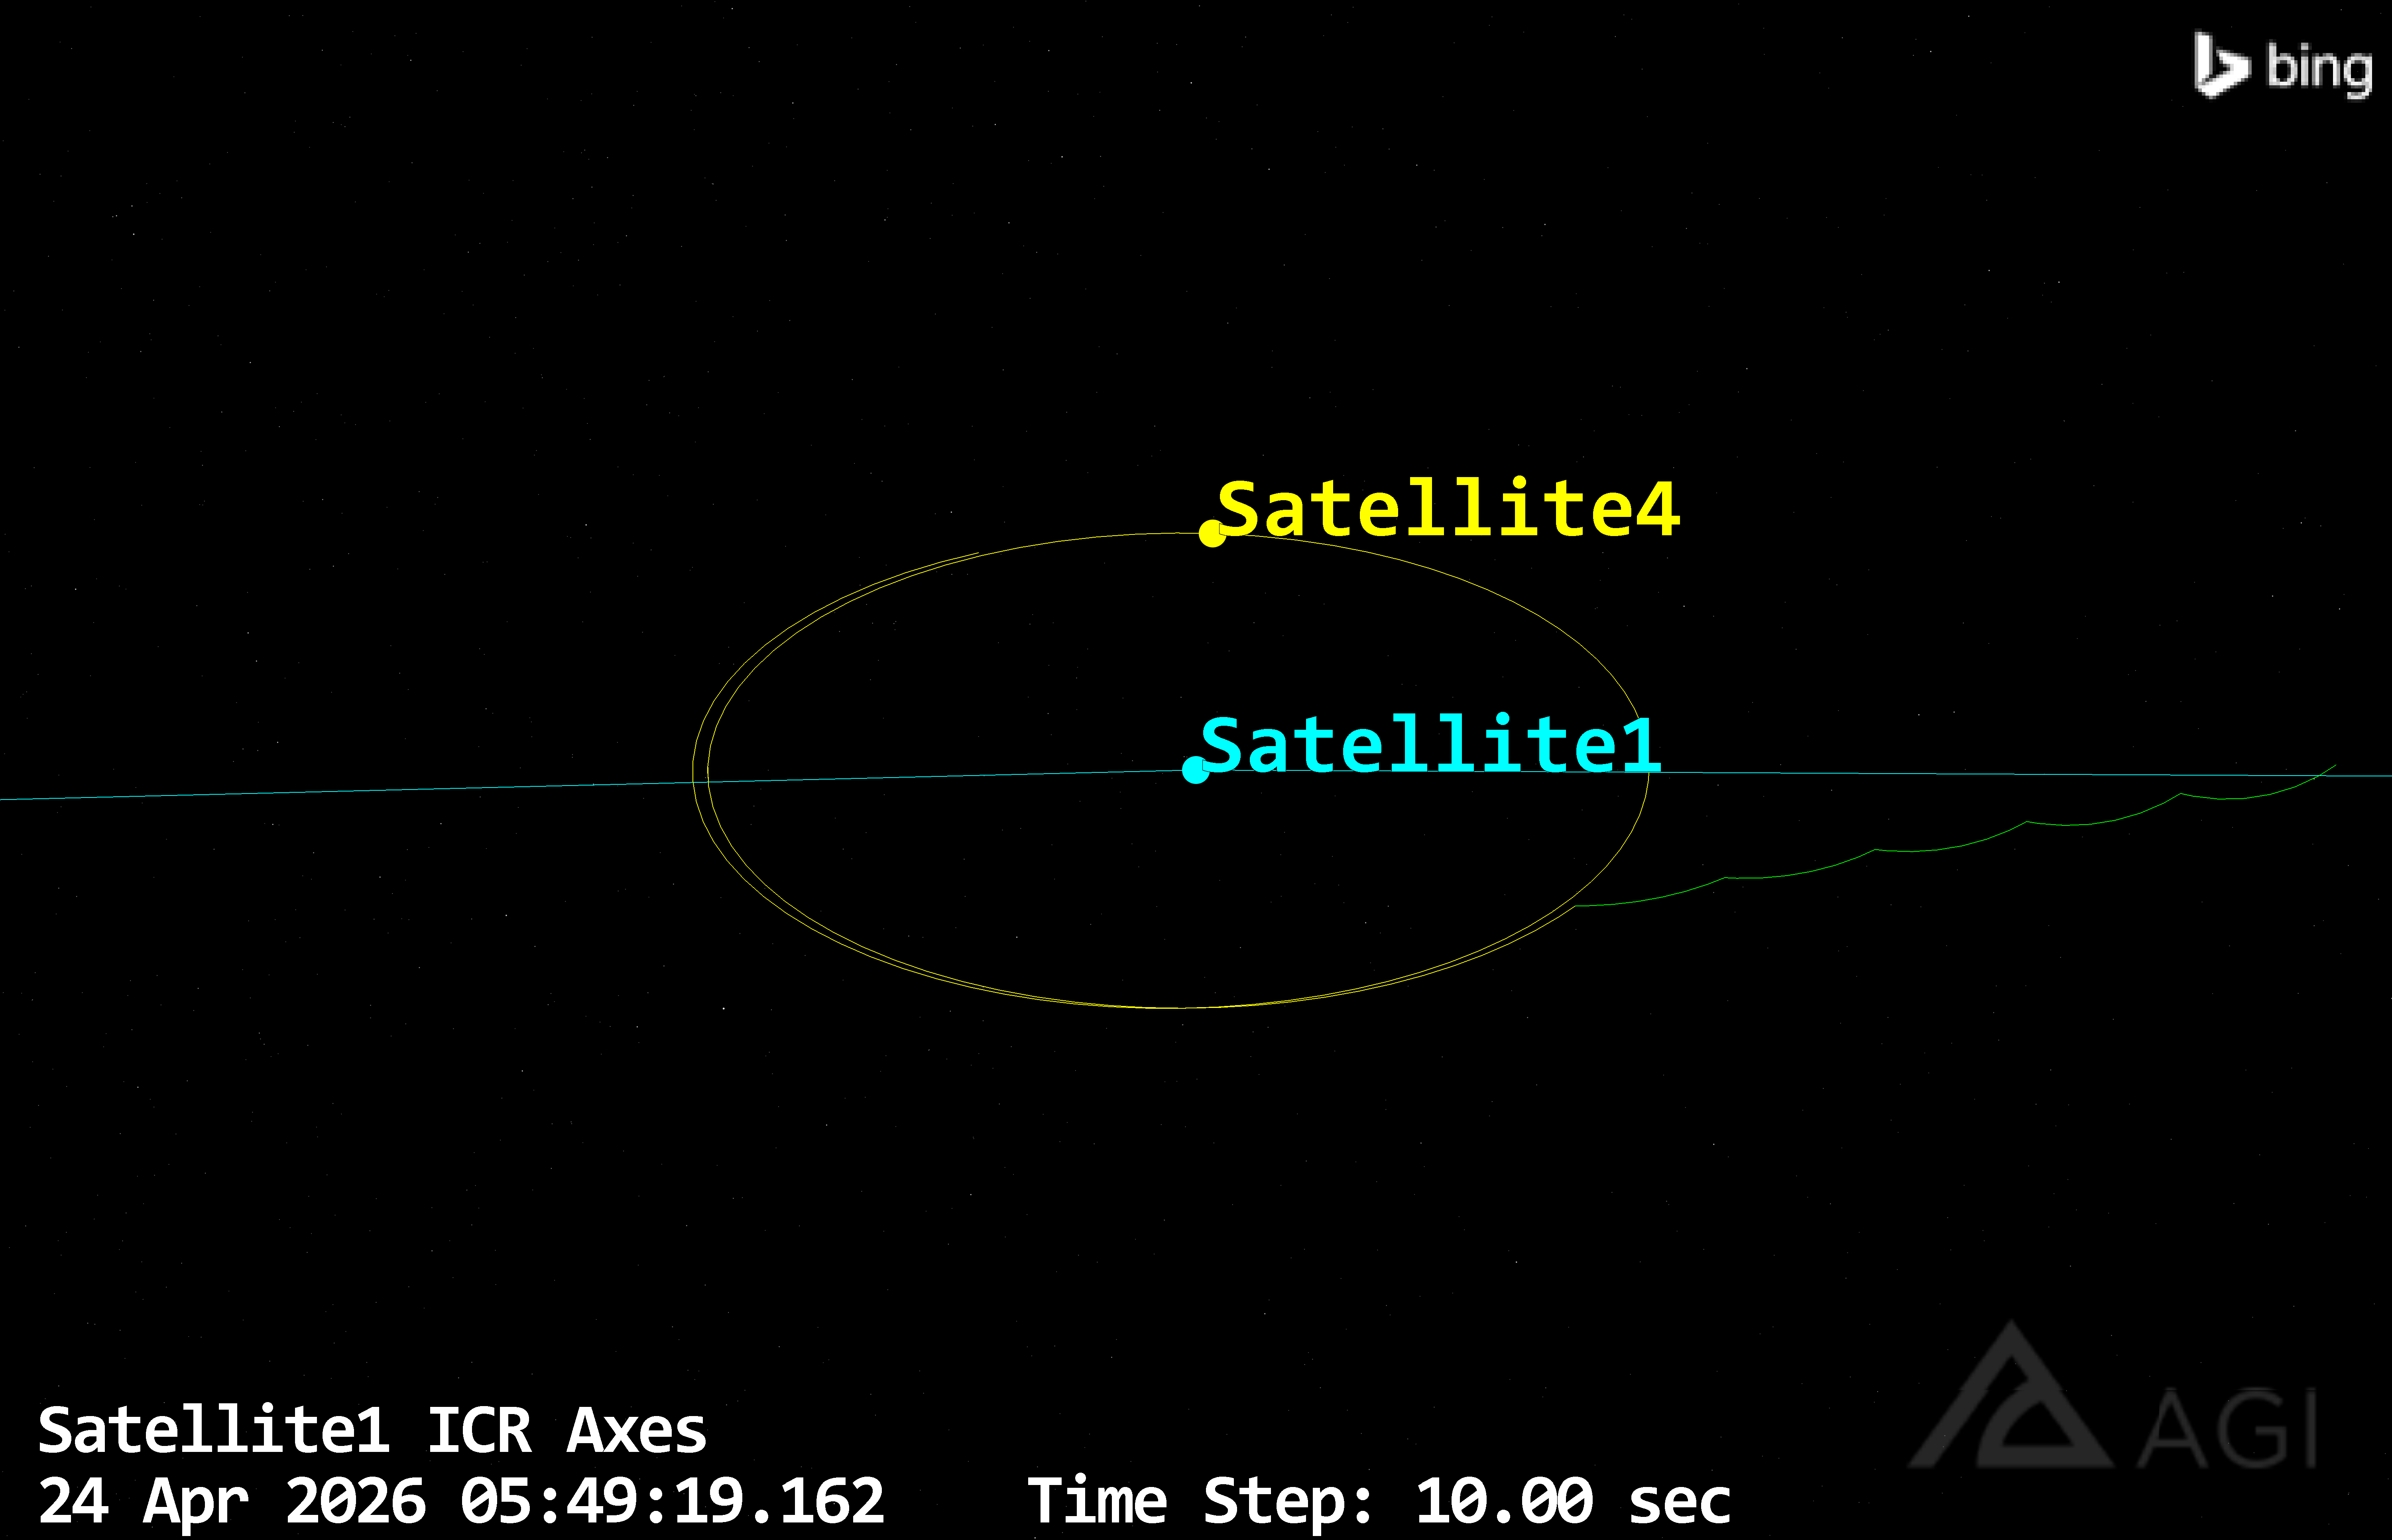
\includegraphics[width=3in]{./image/STK-P-1.png}
  \bicaption[fig:stk-prox]{图}{\centering STK近程导引可视化仿真轨迹}{Fig.}{\centering Visualization of the proximity-guidance transfer trajectory in STK}
\end{figure}
\begin{figure}[t!]
  \centering
  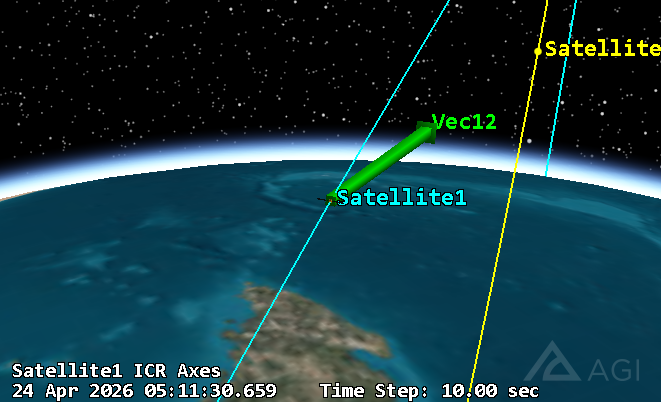
\includegraphics[width=3in]{./image/STK-P-2.png}
  \bicaption[fig:stk-prox-vec]{图}{\centering 卫星相对矢量可视化}{Fig.}{\centering Visualization of the relative vector between the chaser and the target in STK}
\end{figure}

\begin{figure}[t!]
  \centering
  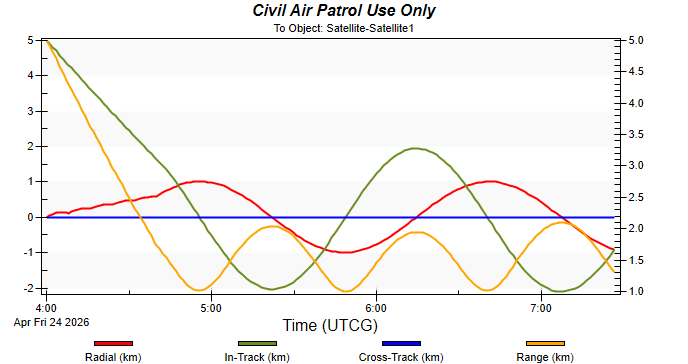
\includegraphics[width=3in]{./image/Satellite4_RIC.png}
  \bicaption[fig:stk-RIP]{图}{\centering 跟踪航天器与目标航天器的位置关系变化}{Fig.}{\centering Relative position change between the chaser and the target in the proximity-guidance phase}
\end{figure}


本文在STK中对转移段数$N=5$的近程导引方案进行了可视化仿真。尽管该方案的总速度增量较$N=2$方案略有增加，但其相对轨迹更贴合参考直线，能够以多次小幅修正实现更平顺的几何逼近，因此本文将其作为近程段的展示与推荐方案。图\ref{fig:stk-prox}展示了跟踪航天器的相对飞行轨迹，可见其在目标附近先沿转移段逐步接近绕飞轨道，随后进入稳定的闭合相对运动。图\ref{fig:stk-prox-vec}展示了卫星相对矢量的可视化，图\ref{fig:stk-RIP}进一步给出了两个航天器的相对位置变化，其中径向和沿迹方向分量先逐段递减，再周期变化，分别对应的抵近阶段与绕飞阶段；而法向分量基本保持为零，说明该方案在数值仿真中保持了本文预设的共面绕飞特征。


\section{结\quad 论}

本文针对目标圆轨道附近的共面抵近任务，完成了远程Lambert转移与近程CW多脉冲导引的建模与结果分析，得到以下结论：

1) 远程段采用二体动力学与零圈Lambert窗口搜索可以有效完成从初始椭圆轨道到目标后方捕获点的转移设计。本文算例中，最优窗口对应出发时刻$t_d=\SI{3960}{s}$、飞行时间$\Delta t=\SI{3300}{s}$，总速度增量为\SI{262.9124}{m/s}；惯性系数值递推所得终点位置误差为\SI{0.001424}{m}，表明远程段解析设计与数值传播结果一致。

% 用于手动调节最后一页的分栏平衡
% \newpage

2) 近程段采用直线指数趋近律与CW状态转移矩阵反解脉冲，可将飞行器由后方捕获点导引至预设平面绕飞轨道。在$N=2,3,4,5$的比较中，随着转移段数增加，最优轨迹的节点数逐渐增多、几何形态更平滑，且对参考直线的贴合程度持续改善；与此同时，总速度增量由\SI{4.3442}{m/s}逐步增加到\SI{6.0034}{m/s}，但其增幅呈逐渐减小趋势。综合考虑速度代价与轨迹形态，本文选取$N=5$方案作为推荐近程转移方案。

3) 近程段参数规律表明，最优切入相位在不同方案下均集中于第三象限，并随转移段数增加整体向较小相位方向偏移；与此同时，$\dot{\rho}_0$与$\dot{\rho}_T$主要决定总转移时间，较小的速率绝对值对应较长的转移时间。因而在该分段导引策略中，切入点相位$\theta_{\mathrm{in}}$是最关键的几何搜索变量，而趋近速率边界更多起到调节时间尺度和限定可行域的作用。


%%%%%%%%%%%%%%%%%%%%%%%%%%%%%%%%%%%%%%%%%%%%%%%%%%%%%%%%%%%%%%%%
% 英文摘要页
%%%%%%%%%%%%%%%%%%%%%%%%%%%%%%%%%%%%%%%%%%%%%%%%%%%%%%%%%%%%%%%%
\newpage
\twocolumn[
  \begin{@twocolumnfalse}\vspace*{1cm}
    \parbox{\textwidth}{
    {\sihao\TimesNMFont\textbf{Simulation of Coplanar Proximity Guidance Based on Lambert Transfer and Clohessy-Wiltshire Equations}}
    \vspace*{0.3cm}

    {\wuhao\TimesNMFont \PrivateAuthorNameEnFull\makebox{$^{\text{1}}$}}\\[0.3cm]
    {\xiaowuhao\textit{\TimesNMFont \PrivateAffiliationEn}}

    \vspace*{2.0cm}

    {
      \TimesNMFont
      \fontsize{9pt}{15pt}\selectfont
      \setlength{\parindent}{0pt}
      \setlength{\parskip}{7.5pt}
      \textbf{Abstract:}
      This paper develops a segmented guidance method for a coplanar proximity mission by combining remote Lambert transfer with proximity multi-impulse guidance based on the CW (Clohessy-Wiltshire) equations. In the remote phase, the chaser is guided from an initial elliptical orbit to a capture point \SI{5}{km} behind the target by using two-body dynamics and Lambert theory, with departure time and time of flight as search variables and the minimum transfer altitude as a safety constraint. In the proximity phase, the transfer from the capture point to a prescribed planar fly-around orbit is designed in the target LVLH frame by using the CW state transition matrix, a straight-line exponential approach law, and the insertion conditions of the reference fly-around orbit. Results show that the optimal remote-guidance window is obtained at $t_d=\SI{3960}{s}$ and $\Delta t=\SI{3300}{s}$, with a total velocity increment of \SI{262.9124}{m/s}; the terminal position error from inertial-frame numerical propagation is \SI{0.001424}{m}. For the proximity phase with $N=2,3,4,5$, the optimal insertion phase remains in the third quadrant and decreases as the number of transfer segments increases. Although the total velocity increment rises from \SI{4.3442}{m/s} to \SI{6.0034}{m/s}, the trajectory becomes progressively closer to the reference straight line and the growth rate of the cost gradually slows down; therefore, the $N=5$ scheme is selected as the recommended compromise between velocity cost and trajectory shape. These results verify the effectiveness of the proposed segmented guidance strategy for coplanar proximity missions.

      \textbf{Keywords:} space proximity; Lambert transfer; Clohessy-Wiltshire equations; multi-impulse guidance; fly-around orbit; LVLH frame
    }
    }
  \end{@twocolumnfalse}
]

\end{document}
